\chapter{Introducción}
\label{chap:antecedentes}

Los programas de computador comerciales para el análisis y diseño de estructuras que se encuentran vigentes a la fecha cuentan, en general, con un entorno gráfico que le permite al usuario describir el modelo de forma interactiva, procesarlo y visualizar los resultados de manera conveniente.\\

En \cite{escamilla1995microcomputadores} se presenta una lista de algunos de estos programas de uso común en América Latina, entre los cuales se encuentra \emph{ETABS} (Three Dimensional Analysis of Building Systems - Extended Version).\\

ETABS es un programa de computador creado por Edward Wilson, Jeffery Hollings y Henry Dovey en 1975. Según \cite{ETABS1975}, este programa de computador fue desarrollado para el análisis estructural lineal de edificios de pórticos y muros a cortante sujetos tanto a cargas estáticas como sísmicas. El edificio es idealizado como un sistema de elementos tipo pórticos y muros a cortante independientes interconectado por losas de entrepiso las cuales son rígidas en su propio plano. \\

Este programa es una extensión de \emph{TABS} (Three Dimensional Analysis of  Building Systems) para poder analizar pórticos en tres dimensiones. Según \cite{ETABS1972}, una de las razones para desarrollar TABS fue darle una retroalimentación a los usuarios de los programas \emph{FRMSTC} (Static Load Analysis of High-Rise Buildings), \emph{FRMDYN} (Dynamic Analysis of Multistory Buildings), \emph{LATERAL} y \emph{SOLID SAP} (Static Analysis Program for Three-Dimensional Solid Structures).\\

FRMSTC permitía analizar edificios simétricos con pórticos y muros a cortante paralelos sujetos a cargas estáticas y evaluar los modos y las frecuencias. FRMDYN era similar a FRMSTC con la excepción que la carga era la aceleración del terreno debido a un desplazamiento dependiente del tiempo. LATERAL fue una extensión de FRMSTC que permitía analizar linealmente pórticos y muros a cortante que no eran necesariamente paralelos con tres grados de libertad en cada piso. SOLID SAP era un programa general de elementos finitos y tenía una opción que permitía introducir la aproximación de piso rígido. Este programa también tenía la opción de realizar análisis dinámico.\\

En la actualidad, ETABS se encuentra en la versión 18.1.1 y según \cite{ETABS2020systemrequirements}, puede ser ejecutado en computadores con sistema operativo Windows 7, Windows 8 o Windows 10 con arquitectura de 64 bits que cuenten como mínimo con un procesador Intel Pentium 4 o AMD Athlon 64, una resolución de 1024x768 pixeles con 16 bits por canal, 8 GB de RAM y 6 GB de espacio en el disco duro. En la figura \ref{fig:etabs_start_page} se presenta la ventana del programa ETABS ejecutándose en un computador con Windows 10.\\

\begin{figure}[ht]
  \centering
  \begin{annotationimage}{width=0.5\textwidth}{introduction/etabs-startup.png}
    \draw[annotation left = {{Barra de título} at 0.91}] to (0.15, 0.81);
    \draw[annotation left = {{Barra de menús} at 0.7}] to (0.15, 0.8);
    \draw[annotation left = {{Explorador del modelo} at 0.5}] to (0.18, 0.65);
    \draw[annotation left = {{Barra de herramientas} at 0.3}] to (0.15, 0.4);
    \draw[annotation left = {{Barra de estado} at 0.125}] to (0.15, 0.225);
    \draw[annotation right = {{Barra de herramientas} at 0.655}] to (0.84, 0.765);
    \draw[annotation right = {{Vista del modelo} at 0.47}] to (0.75, 0.67);
    \draw[annotation right = {{Indicador de actualizaciones} at 0.86}] to (0.85, 0.76);
  \end{annotationimage}
  \caption{Ventana del programa ETABS ejecutandose en Windows 10.}
  \label{fig:etabs_start_page}
\end{figure}

A través de múltiples cuadros de diálogo, los cuales son accesibles ya sea a través de la barra de menús, las barras de herramientas, el explorador del modelo, las vistas del modelo o con atajos de teclado, el usuario es capaz de modelar la estructura que desea analizar al describir los materiales, las secciones transversales, los elementos estructurales, las condiciones de apoyo, los diafragmas y las cargas. \\

Según \cite{ETABS2017analysisreferencemanual}, ETABS analiza el modelo usando el motor de análisis \emph{SAPFire}, el cual es común a otros programas de la misma compañia (\emph{SAP2000}, \emph{SAFE} y \emph{CSiBridge}). SAPFire es la última versión de la serie de programas \emph{SAP} y ofrece las siguientes herramientas:
\begin{itemize}
\item Análisis estático y dinámico,
\item Análisis lineal y no lineal,
\item Análisis sísmico y análisis incremental no lineal (\emph{pushover}),
\item Análisis de cargas móviles,
\item No linealidad geométrica, incluyendo efectos P-delta y grandes desplazamientos,
\item Etapas constructivas,
\item Fluencia lenta (\emph{creep}), retracción (\emph{shrinkage}) y envejecimiento,
\item Análisis de pandeo,
\item Análisis de densidad espectral de potencia y estado estacionario,
\item Elementos tipo pórtico y laminares, incluyendo el comportamiento de vigas, columnas, cerchas, membranas y placas,
\item Elementos tipo cable y tendón,
\item Elementos bidimensionales planos y elementos sólidos asimétricos,
\item Elementos sólidos tridimensionales,
\item Resortes no lineales y apoyos,
\item Propiedades de los resortes y apoyos dependientes de la frecuencia,
\end{itemize}

Con los resultados del análisis del modelo, el posprocesador de ETABS puede \emph{diseñar} los elementos estructurales de acuerdo a uno de varios códigos de diseño de diferentes países. ETABS es capaz de diseñar pórticos en acero, pórticos en concreto, vigas compuestas, columnas compuestas, vigas en acero de alma abierta (\emph{steel joist}), muros a cortpante y losas de concreto.\\

Adicionalmente, según \cite{ETABS2019welcome}, ETABS cuenta con la posibilidad de generar dibujos estructurales esquemáticos de las plantas estructurales, de los despieces de vigas, columnas y muros a cortante, y de los detalles de las conexiones de acero.\\

En términos generales, estos programas de computador comerciales cuenta con características similares a las de ETABS. Actualmente, dichos programas están innovando para permitirle al usuario trabajar con modelos \emph{BIM} (Building Information Modeling).\\

\section{Objetivo}

Desarrollar un programa de computador a código abierto para el análisis de estructuras tridimensionales tipo pórtico sometidas a cargas estáticas.\\

Con este trabajo se pretende contribuir al ejercicio libre de la profesión del ingeniero estructural y a la enseñanza del análisis de las estructuras.

\subsection{Objetivos específicos}

\begin{itemize}
\item Desarrollar el ambiente gráfico y la interfaz gráfica de usuario del programa de computador para permitirle al usuario ingresar los datos que describen la estructura, las acciones a las cuales se encuentra sometida y visualizar los resultados del análisis estructural.
\item Desarrollar el módulo de análisis estructural para calcular el desplazamiento de los nudos, el valor de las reacciones y de las fuerzas internas de los elementos de una estructura sometida a cargas estáticas.
\end{itemize}

\section{Metodología}

Se desarrollaron los programas de computador \emph{pyFEM} y \emph{FEM.js}. El primero para analizar estructuras tridimensionales tipo pórtico sometidas a cargas estáticas y el segundo para modelarlas. Esto con el fin que FEM.js pueda ser usado junto con otro programa de computador diferente a pyFEM.\\

Durante el desarrollo de estos programas, así como el de este documento, se utilizó \emph{git} como sistema de control de versiones. Según \cite{chacon2014git}, git es un sistema distribuido de control de versiones que registra los cambios realizados a un conjunto de archivos para coordinar el trabajo entre programadores.\\

Una copia de los repositorios de pyFEM y FEM.js se encuentran en la página de internet \emph{GitHub}, la cual permite alojar proyectos utilizando git. pyFEM está alojado en \url{https://github.com/rvcristiand/pyFEM} mientras que FEM.js está alojado en \url{https://github.com/rvcristiand/FEM.js}.\\

\subsection{pyFEM}

pyFEM fue desarrollado en \emph{Python}. Según \cite{lutz2013python}, Python es un lenguaje de programación interpretado orientado a objetos cuya filosofía hace enfasis en la legibilidad de su código. Los archivos revelantes que componen el repositorio de pyFEM son:
\pagebreak

\dirtree{%
  .1 pyFEM/.
  .2 LICENSE.
  .2 README.md.
  .2 example\_1.json.
  .2 example\_2.json.
  .2 example\_3.json.
  .2 pyFEM/.
  .3 classtools.py.
  .3 core.py.
  .3 primitives.py.
  .2 test/.
  .3 space\_frame.py.
  .3 trusses.py.
}

\bigskip
El archivo \verb|LICENCE| contiene la licencia de pyFEM, la cual se presenta a continuación.

\begin{quotation}
  The MIT License\\

  Copyright (c) 2019 pyFEM\\

  Permission is hereby granted, free of charge, to any person obtaining a copy of this software and associated documentation files (the "Software"), to deal in the Software without restriction, including without limitation the rights to use, copy, modify, merge, publish, distribute, sublicense, and/or sell copies of the Software, and to permit persons to whom the Software is furnished to do so, subject to the following conditions:\\
  
  The above copyright notice and this permission notice shall be included in all copies or substantial portions of the Software.\\

  THE SOFTWARE IS PROVIDED ``AS IS'', WITHOUT WARRANTY OF ANY KIND, EXPRESS OR IMPLIED, INCLUDING BUT NOT LIMITED TO THE WARRANTIES OF MERCHANTABILITY, FITNESS FOR A PARTICULAR PURPOSE AND NONINFRINGEMENT. IN NO EVENT SHALL THE AUTHORS OR COPYRIGHT HOLDERS BE LIABLE FOR ANY CLAIM, DAMAGES OR OTHER LIABILITY, WHETHER IN AN ACTION OF CONTRACT, TORT OR OTHERWISE, ARISING FROM, OUT OF OR IN CONNECTION WITH THE SOFTWARE OR THE USE OR OTHER DEALINGS IN THE SOFTWARE.
\end{quotation}

El archivo \verb|README.md| contiene todas las instrucciones necesarias para ejecutar y usar pyFEM.\\

% TODO: hacer el README.md
% Como se instala el programa

La carpeta \emph{pyFEM} contiene los archivos \verb|classtools.py|, \verb|core.py| y \verb|primitives.py| los cuales contienen las instrucciones para analizar los modelos. La extensión \emph{py} se usa para indicar que los archivos son programas de Python.\\

En el archivo \verb|classtools.py| se encuentran las \emph{clases} \verb|UniqueInstances| y \verb|AttrDisplay|, la primera para evitar que se creen \emph{objetos} de una misma clase con la misma información y la segunda para generar una representación conveniente de los objetos.\\

En el archivo \verb|primitives.py| se encuentran varias clases, entre ellas \verb|Material|, \verb|Section|, \verb|Joint|, \verb|Frame|, \verb|Support|, \verb|LoadPattern|, etc., las cuales permiten describir los diferentes atributos del modelo.\\

En el archivo \verb|core.py| se encuentra la clase \verb|Structure| la cual permite describir estructuras para ser analizados. Para crear objetos de esta clase se debe llamar la clase indicando los grados de libertad a tener en cuenta. A partir de un objeto de esta clase es posible describir el modelo de la estructura al agregar materiales, secciones transversales, nodos, elemenetos tipo pórtico, apoyos, patrones de carga, cargas en los nodos y cargas distribuidas en los elementos tipo pórtico.\\

Los archivos \verb|example_1.json|, \verb|example_2.json| y \verb|example_3.json| almacenan los modelos de tres de los ejemplos presentados en \cite{escamilla1995microcomputadores} que han sido analizados con pyFEM. La extensión \emph{json} se usa para indicar que los archivos tienen formato \emph{JSON} (de sus siglas en inglés JavaScript Object Notation), el cual es un formato sencillo para el intercambio de datos. El modelo es descrito de tal manera que puede ser interpretado por FEM.js para generar su representación en una escena tridimensional. \\

En el ejemplo \ref{ej:cercha-plana} se presenta la solución a un ejercicio de \cite{escamilla1995microcomputadores} usando pyFEM. En el capítulo \ref{cha:pyFEM} se presentan las rutinas que ejecuta pyFEM para solucionar los modelos estructurales.\\
% \pagebreak

\begin{ejemplo}
  \label{ej:cercha-plana}
  Resuelva completamente la cercha mostrada por el método matricial de los desplazamientos. El material es acero estructural con $ E = 2040\; t / cm^2 $. Las áreas están dadas entre paréntesis en $ cm^2 $.\\
  
  \begin{center}
    \begin{tikzpicture}
      % Points
      \point{1}{0}{0};
      \point{2}{8}{0};
      \point{3}{4}{3};
      \point{4}{4}{0};
      
      \point{p}{4}{-1.3};
      \point{q}{5.05}{3.7875};
      
      \point{1-3}{2}{1.5};
      \point{1-4}{2}{0};
      \point{3-2}{6}{1.5};
      \point{4-2}{6}{0};
      \point{4-3}{4}{1.5};
      
      % Beams
      \beam{2}{1}{3}[0][0];
      \beam{2}{1}{4}[1][1];
      \beam{2}{3}{2}[1][1];
      \beam{2}{4}{2}[1][1];
      \beam{2}{4}{3}[1][1];
      
      % Supports
      \support{1}{1};
      \support{2}{2};
      
      % Joints
      \hinge{1}{1};
      \hinge{1}{2};
      \hinge{1}{3};
      \hinge{1}{4};
      
      % Loads
      \load{1}{q}[216.87];
      \load{1}{p}[90];
      
      % notation
      \notation{1}{1}{1}[above left];
      \notation{1}{2}{2}[above right];
      \notation{1}{3}{3}[above left];
      \notation{1}{4}{4}[below left];
      
      \notation{1}{3}{$ \SI{5}{\tonne} $}[above right=10mm];
      \notation{1}{4}{$ \SI{20}{\tonne} $}[below right=5mm and 0mm];
      
      \notation{5}{1}{3}[$ (100) $ ][.5][above][0.5];
      \notation{5}{1}{4}[$ (40) $ ][.5][above][0.5];
      \notation{5}{3}{2}[$ (150) $ ][.5][above][0.5];
      \notation{5}{4}{2}[$ (40) $ ][.5][above][0.5];
      \notation{5}{4}{3}[$ (30) $ ][.5][right][1];
            
      % Dimensions
      \dimensioning{1}{1}{4}{-1.5}[$ \SI{4}{m} $];
      \dimensioning{1}{4}{2}{-1.5}[$ \SI{4}{m} $];
      \dimensioning{2}{2}{3}{9}[$ \SI{3}{m} $];
    \end{tikzpicture}
    \captionof{figure}{Cercha simple plana del \textit{Ejemplo 7.1} de \cite{escamilla1995microcomputadores}.}
  \end{center}

  \emph{\textbf{Solución -}} En el algoritmo \ref{alg:cercha_plana} se presenta un programa de Python para analizar el modelo de la estructura usando pyFEM. Las instrucciones consisten en crear un nuevo objeto tipo \verb|Structure|, al cual se le ha dado el nombre \emph{model}, agregarle
  \begin{inparaenum}[$ (a) $]
  \item materiales,
  \item secciones transversales,
  \item nodos,
  \item elementos tipo pórtico,
  \item apoyos, patrones de carga y
  \item cargas en los nodos,
  \end{inparaenum}
  analizar el modelo y exportarlo a formato JSON.\\

  Cuando se ejecuta la instrucción \verb|model.solve()| pyFEM comienza a solucionar el modelo de la estructura. Los pasos que efectúa para solucionar el modelo son:
  \begin{inparaenum}[$ (1) $]
  \item asignar los grados de libertad de los nodos, 
  \item ensamblar la matriz de rigidez del modelo de la estructura, 
  \item imponer las condiciones de apoyo en la matriz de rigidez del modelo, 
  \item ensamblar el vector de fuerzas en los nodos para cada uno de los patrones de carga, 
  \item imponer las condiciones de apoyo en el vector de fuerzas en los nodos para cada caso de carga, 
  \item encontrar los desplazamientos de los nodos para cada patrón de carga, 
  \item encontrar las reacciones en los apoyos para cada patrón de carga y
  \item guardar la solución en los nodos y en los apoyos para cada patrón de carga.
  \end{inparaenum} \\
  
  % \begin{minipage}{\textwidth}
  \begin{lstlisting}[language=Python,caption=Ingreso de los datos del modelo de la estructura a \textit{pyFEM}.,label=alg:cercha_plana, frame=single]
# create the model
model = Structure(ux=True, uy=True)

# add materials
model.add_material(key='1', modulus_elasticity=2040e4)

# add sections
model.add_section(key='1', area=030e-4)
model.add_section('2', area=040e-4)
model.add_section('3', area=100e-4)
model.add_section('4', area=150e-4)

# add joints
model.add_joint(key=1, x=0, y=0)
model.add_joint(2, 8, 0)
model.add_joint(3, 4, 3)
model.add_joint(4, 4, 0)

# add frames
model.add_frame(key='1-3', key_joint_j=1, key_joint_k=3, key_material='1', key_section='3')
model.add_frame('1-4', 1, 4, '1', '2')
model.add_frame('3-2', 3, 2, '1', '4')
model.add_frame('4-2', 4, 2, '1', '2')
model.add_frame('4-3', 4, 3, '1', '1')

# add supports
model.add_support(key_joint=1, ux=True, uy=True)
model.add_support(2, ux=False, uy=True)

# add load patterns
model.add_load_pattern(key='point loads')

# add point loads
model.add_load_at_joint(key_load_pattern='point loads', key_joint=3, fx=5 * 0.8, fy=5 * 0.6)
model.add_load_at_joint('point loads' , 4, fy=-20)

# solve the problem
model.solve()

print(model)

# export the model
model.export('example_1.json')
  \end{lstlisting}
% \end{minipage}

  Para realizar el ensamblaje de la matriz de rigidez del modelo de la estructura y del vector de fuerzas de los nodos, pyFEM asigna números a los grados de libertad de los nodos de la estructura en el orden en que fueron ingresados; al nodo 1 se le han asignado los grados de libertad \emph{0} y \emph{1}, al nodo 2 los grados de libertad \emph{2} y \emph{3}, y así sucesivamente.\\

  Una vez se establecen los grados de libertad de los nodos se ensambla la matriz de rigidez del modelo de la estructura. Este proceso consiste en calcular una a una las matrices de rigidez de los elementos ensamblandolas en la matriz de rigidez del modelo.\\

  El usuario puede consultar las matrices de rigidez de cada uno de los elementos del modelo de la estructura. En \ref{eq:matriz-rigidez-elemento-portico-coordenadas-locales} se presenta la matriz de rigidez en coordenadas locales del elemento 1-3, la cual se obtiene mediante la instrucción \verb|model.frames['1-3'].get_local_stiffness_matrix()|.\\

  \begin{equation}
    \label{eq:matriz-rigidez-elemento-portico-coordenadas-locales}
    \begin{bNiceArray}{CCCCC}
      40800 & 0 & -40800 & 0\\
      0 & 0 &      0 & 0\\
      -40800 & 0 & 40800 & 0\\
      0 & 0 &      0 & 0\\
    \end{bNiceArray}
    \si[per-mode=symbol]{\tonne\per\meter}
  \end{equation}

  Así mismo, el usuario puede consultar las matrices de rotación de cada uno de los elementos del modelo. En \ref{eq:matriz-rotacion} se presenta la matriz de rotación del elemento 1-3, la cual se obtiene mendiante la instrucción \verb|model.frames['1-3'].get_rotation_matrix()|.\\

  \begin{equation}
    \label{eq:matriz-rotacion}
    \begin{bNiceArray}{CCCCC}
      0.8 & -0.6 &   0 &    0\\
      0.6 &  0.8 &   0 &    0\\
      0 &    0 & 0.8 & -0.6\\
      0 &    0 & 0.6 &  0.8\\
    \end{bNiceArray}
  \end{equation}

  El usuario tambien puede consultar las matrices de rigidez en coordenadas globales de cada uno de los elementos del modelo de la estructura. En \ref{eq:matriz-rigidez-elemento-portico-coordenadas-globales} se presenta la matriz de rigidez en coordenadas globales del elemento 1-3, con sus respectivos grados de libertad, la cual se obtiene mediante la instrucción \verb|model.frames['1-3'].get_global_stiffness_matrix()|.

  \begin{equation}
    \label{eq:matriz-rigidez-elemento-portico-coordenadas-globales}
    \begin{bNiceArray}{CCCCC}[
        first-row,
        first-col,
      ]
      & \emph{0} & \emph{1} & \emph{4} & \emph{5}\\
      \emph{0} & 26112 & 19584 & -261112 & -19584\\
      \emph{1} & 19584 & 14688 & -19584 & -14688\\
      \emph{4} & -26112 & -19584 & 26112 & 19584\\
      \emph{5} & -19584 & -14688 & 19584 & 14688\\
    \end{bNiceArray}
    \si[per-mode=symbol]{\tonne\per\meter}
  \end{equation}

  En \ref{eq:k_1_4}, \ref{eq:k_3_2} y \ref{eq:k_4_3} se presentan las matrices de rigidez en coordenadas globales de los elementos 1-4, 3-2 y 4-3 de la estructura las cuales se obtienen con instrucciones similares a la anterior.\\

  \begin{equation}
    \begin{bNiceArray}{CCCCC}[
        first-row,
        first-col,
      ]
      \label{eq:k_1_4}
      & \emph{0} & \emph{1} & \emph{6} & \emph{7}\\
      \emph{0} & 20400 & 0 & -20400 & 0\\
      \emph{1} & 0 & 0 & 0 & 0\\
      \emph{6} & -20400 & 0 & 20400 & 0\\
      \emph{7} & 0 & 0 & 0 & 0 \\
    \end{bNiceArray}
    \si[per-mode=symbol]{\tonne\per\meter}
  \end{equation}

  \begin{equation}
    \begin{bNiceArray}{CCCCC}[
        first-row,
        first-col,
      ]
      \label{eq:k_3_2}    
      & \emph{4} & \emph{5} & \emph{2} & \emph{3}\\
      \emph{4} & 39168 & -29376 & -39168 & 29376\\
      \emph{5} & -29376 & 22032 & 29376 & -22032\\
      \emph{2} & -39168 & 29376 & 39168 & -29376\\
      \emph{3} & 29376 & -22032 & -29376 & 22032\\
    \end{bNiceArray}
    \si[per-mode=symbol]{\tonne\per\meter}
  \end{equation}

  \begin{equation}
    \begin{bNiceArray}{CCCCC}[
        first-row,
        first-col,
      ]
      \label{eq:k_4_3}
      & \emph{6} & \emph{7} & {4} & \emph{5}\\
      \emph{6} & 0 & 0 & 0 & 0\\
      \emph{7} & 0 & 20400 & 0 & -20400\\
      \emph{4} & 0 & 0 & 0 & 0\\
      \emph{5} & 0 & -20400 & 0 & 20400\\
    \end{bNiceArray}
    \si[per-mode=symbol]{\tonne\per\meter}
  \end{equation}

  El usuario también puede consultar la matriz de rigidez del modelo de la estructura mediante la instrucción \verb|structure.get_stiffness_matrix()|. En \ref{eq:k_global} se presenta la matriz de rigidez de la estructura.\\

  \begin{equation}
    \begin{bNiceArray}{CCCCCCCC}[
        first-row,
        first-col,
      ]
      & \emph{0} & \emph{1} & \emph{2} & \emph{3} & \emph{4} & \emph{5} & \emph{6} & \emph{7}\\
      \emph{0} &  46512 &  19584 &      0 &      0 & -26112 & -19584 & -20400 &      0\\
      \emph{1} &  19584 &  14688 &      0 &      0 & -19584 & -14688 &      0 &      0\\
      \emph{2} &      0 &      0 &  59568 & -29376 & -39168 &  29376 & -20400 &      0\\
      \emph{3} &      0 &      0 & -29376 &  22032 &  29376 & -22032 &      0 &      0\\
      \emph{4} & -26112 & -19584 & -39168 &  29376 &  65280 &  -9792 &      0 &      0\\
      \emph{5} & -19584 & -14688 &  29376 & -22032 &  -9792 &  57120 &      0 & -20400\\
      \emph{6} & -20400 &      0 & -20400 &      0 &      0 &      0 &  40800 &      0\\
      \emph{7} &      0 &      0 &      0 &      0 &      0 & -20400 &      0 &  20400
      \label{eq:k_global}
    \end{bNiceArray}
    \si[per-mode=symbol]{\tonne\per\meter}
  \end{equation}

  Una vez se ensambla la matriz de rigidez del modelo se modifica para tener en cuenta las condiciones de apoyo. Este proceso consiste en modificar las filas y las columnas asociadas a los grados de libertad restringidos. En \ref{eq:k_global_support_applied} se presenta la matriz de rigidez sujeta a las condiciones de apoyo del modelo de la estructura la cual se obtiene mediante la instrucción \verb|model.get_stiffness_matrix_with_support()|.\\

  \begin{equation}
    \label{eq:k_global_support_applied}
    \begin{bNiceArray}{CCCCCCCC}[
        first-row,
        first-col,
      ]
      & \emph{0} & \emph{1} & \emph{2} & \emph{3} & \emph{4} & \emph{5} & \emph{6} & \emph{7}\\
      \emph{0} & 1 & 0 &      0 & 0 &      0 &      0 &      0 &      0\\
      \emph{1} & 0 & 1 &      0 & 0 &      0 &      0 &      0 &      0\\
      \emph{2} & 0 & 0 &  59568 & 0 & -39168 &  29376 & -20400 &      0\\
      \emph{3} & 0 & 0 &      0 & 1 &      0 &      0 &      0 &      0\\
      \emph{4} & 0 & 0 & -39168 & 0 &  65280 &  -9792 &      0 &      0\\
      \emph{5} & 0 & 0 &  29376 & 0 &  -9792 &  57120 &      0 & -20400\\
      \emph{6} & 0 & 0 & -20400 & 0 &      0 &      0 &  40800 &      0\\
      \emph{7} & 0 & 0 &      0 & 0 &      0 & -20400 &      0 &  20400
    \end{bNiceArray}
    \si[per-mode=symbol]{\tonne\per\meter}
  \end{equation}

  Una vez se obtiene la matriz de rigidez modificada del modelo de la estructura se resuelve para cada uno de los patrones de carga.\\

  Así como se deben encontrar las matrices de rigidez de cada uno de los elementos del modelo de la estructura para posteriormente ensamblarlas, se debe encontrar la acción en los nodos de cada carga. En \ref{eq:f_global} se presenta el vector de fuerzas nodales del modelo para el patrón de carga \emph{point loads} mediante la instrucción \verb|structure.load_patterns['point loads'].get_f()|.\\

  \begin{equation}
    \label{eq:f_global}
    \begin{BNiceArray}{CC}[
        first-col,
      ]
      \emph{0} & 0\\
      \emph{1} & 0\\
      \emph{2} & 0\\
      \emph{3} & 0\\
      \emph{4} & 4\\
      \emph{5} & 3\\
      \emph{6} & 0\\
      \emph{7} & -20
    \end{BNiceArray}
    \si{\tonne}
  \end{equation}

  \bigskip
  Obtenido el vector de fuerzas para dicho patrón de carga se imponen las condiciones de apoyo del modelo de la estructura. Debido a que los desplazamiento en los apoyos son iguales a cero el vector de fuerzas en los nodos no varia.\\

  Al contar con la matriz de rigidez y el vector de fuerzas en los nodos, ambos modificados por las condiciones de apoyo, se calculan los desplazamientos y las reacciones. En \ref{eq:u_point_loads} y \ref{eq:f_point_loads_solution} se presentan el vector de desplazamientos y el vector de fuerzas en los nodos del modelo de la estructura para el patrón de carga \textit{point loads}, los cuales son iguales a los presentados en \cite{escamilla1995microcomputadores}.

  \begin{equation}
    \label{eq:u_point_loads}
    \begin{BNiceArray}{CC}[
        first-col,
      ]
      \emph{0} & 0\\
      \emph{1} & 0\\
      \emph{2} & 1.307\\
      \emph{3} & 0\\
      \emph{4} & 0.645\\
      \emph{5} & -1.337\\
      \emph{6} & 0.654\\
      \emph{7} & -2.317\\
    \end{BNiceArray}
    \SI{1e-3}{\meter}
  \end{equation}

  \begin{equation}
    \label{eq:f_point_loads_solution}
    \begin{BNiceArray}{CC}[
        first-col,
      ]
      \emph{0} & -4\\
      \emph{1} & 7\\
      \emph{2} & 0\\
      \emph{3} & 10\\
      \emph{4} & 4\\
      \emph{5} & 3\\
      \emph{6} & 0\\
      \emph{7} & -20
    \end{BNiceArray} 
    \si{\tonne} 
  \end{equation}

  Cuando se ejecuta la instrucción \verb|print(model)| pyFEM genera un informe del análisis. A continuación se presenta el informe generado para el objecto \verb|model|.\\

  \begin{lstlisting}[language={}, frame=single]
Flag joint displacements
------------------------
ux: True
uy: True
uz: False
rx: False
ry: False
rz: False

Materials
---------
label   E                       G
1               20400000.0,     0

Sections
--------
label   A               Ix      Iy      Iz
1               0.003,  0,      0,      0
2               0.004,  0,      0,      0
3               0.01,   0,      0,      0
4               0.015,  0,      0,      0

Joints
------
label   x       y       z
1               0,      0,      0
2               8,      0,      0
3               4,      3,      0
4               4,      0,      0

Frames
------
label   Joint j Joint k material        section
1-3             1               3               1                       3
1-4             1               4               1                       2
3-2             3               2               1                       4
4-2             4               2               1                       2
4-3             4               3               1                       1

Supports
--------
label   ux              uy              uz              rx              ry              rz
1               True,   True,   False,  False,  False,  False
2               False,  True,   False,  False,  False,  False

Load patterns
-------------
point loads:
label        fx        fy        fz        mx        my        mz
3              4.0       3.0         0         0         0         0
4                0       -20         0         0         0         0

Displacements
-------------
point loads:
label         ux         uy         uz         rx         ry         rz
1               +0.00000,       +0.00000,       +0.00000,       +0.00000,       +0.00000,       +0.00000
2               +0.00131,       +0.00000,       +0.00000,       +0.00000,       +0.00000,       +0.00000
3               +0.00065,       -0.00134,       +0.00000,       +0.00000,       +0.00000,       +0.00000
4               +0.00065,       -0.00232,       +0.00000,       +0.00000,       +0.00000,       +0.00000

Reactions
---------
point loads:
label         fx         fy         fz         mx         my         mz
1               -4.00000,       +7.00000,       +0.00000,       +0.00000,       +0.00000,       +0.00000
2               +0.00000,       +10.00000,      +0.00000,       +0.00000,       +0.00000,       +0.00000
  \end{lstlisting}

  Cuando se ejecuta la instrucción \verb|model.export('example_1.json')| pyFEM genera un archivo que contiene toda la información del modelo en formato JSON para ser leído por FEM.js. A continuación se presenta la información del modelo en formato JSON.\\
  \begin{lstlisting}[language={}, frame=single]
{
    "materials": {
        "1": {
            "E": 20400000.0,
            "G": 0
        }
    },
    "sections": {
        "1": {
            "area": 0.003,
            "Ix": 0,
            "Iy": 0,
            "Iz": 0,
            "type": "Section"
        },
        "2": {
            "area": 0.004,
            "Ix": 0,
            "Iy": 0,
            "Iz": 0,
            "type": "Section"
        },
        "3": {
            "area": 0.01,
            "Ix": 0,
            "Iy": 0,
            "Iz": 0,
            "type": "Section"
        },
        "4": {
            "area": 0.015,
            "Ix": 0,
            "Iy": 0,
            "Iz": 0,
            "type": "Section"
        }
    },
    "joints": {
        "1": {
            "x": 0,
            "y": 0,
            "z": 0
        },
        "2": {
            "x": 8,
            "y": 0,
            "z": 0
        },
        "3": {
            "x": 4,
            "y": 3,
            "z": 0
        },
        "4": {
            "x": 4,
            "y": 0,
            "z": 0
        }
    },
    "frames": {
        "1-3": {
            "j": 1,
            "k": 3,
            "material": "1",
            "section": "3"
        },
        "1-4": {
            "j": 1,
            "k": 4,
            "material": "1",
            "section": "2"
        },
        "3-2": {
            "j": 3,
            "k": 2,
            "material": "1",
            "section": "4"
        },
        "4-2": {
            "j": 4,
            "k": 2,
            "material": "1",
            "section": "2"
        },
        "4-3": {
            "j": 4,
            "k": 3,
            "material": "1",
            "section": "1"
        }
    },
    "supports": {
        "1": {
            "ux": true,
            "uy": true,
            "uz": false,
            "rx": false,
            "ry": false,
            "rz": false
        },
        "2": {
            "ux": false,
            "uy": true,
            "uz": false,
            "rx": false,
            "ry": false,
            "rz": false
        }
    },
    "load_patterns": {
        "point loads": {
            "joints": {
                "3": [
                    {
                        "fx": 4.0,
                        "fy": 3.0,
                        "fz": 3.0,
                        "mx": 0,
                        "my": 0,
                        "mz": 0
                    }
                ],
                "4": [
                    {
                        "fx": 0,
                        "fy": -20,
                        "fz": -20,
                        "mx": 0,
                        "my": 0,
                        "mz": 0
                    }
                ]
            }
        }
    }
}
  \end{lstlisting}    
\end{ejemplo}

\subsection{FEM.js}

FEM.js fue desarrollado en \emph{Three.js}. Según \cite{dirksen2015threejs}, Three.js es un \emph{API} (de sus siglas en inglés \emph{application programming interface}) programada en \emph{JavaScript} para \emph{WebGL} que permite crear escenas tridimensionales en el navegador de internet. Los archivos revelantes que componen el repositorio de FEM.js son:
\bigskip

\dirtree{%
  .1 FEM.js/.
  .2 LICENSE.
  .2 README.md.
  .2 css/.
  .3 style.css.
  .2 example\_1.json.
  .2 example\_2.json.
  .2 example\_3.json.
  .2 index.html.
  .2 libs/.
  .3 CSS2DRenderer.js.
  .3 OrbitControls.js.
  .3 Projector.js.
  .3 dat.gui.min.js.
  .3 stats.js.
  .3 three.js.
  .2 main.js.
  .2 modules/.
  .3 FEM.js.
  .3 terminal.js.
}
  
\bigskip

El archivo \verb|LICENCE| contiene la licencia de FEM.js, la cual se presenta a continuación.

\begin{quotation}
  THE MIT License\\

  Copyright (c) 2020 FEM.js\\

  Permission is hereby granted, free of charge, to any person obtaining a copy of this software and associated documentation files (the "Software"), to deal in the Software without restriction, including without limitation the rights to use, copy, modify, merge, publish, distribute, sublicense, and/or sell copies of the Software, and to permit persons to whom the Software is furnished to do so, subject to the following conditions:\\
  
  The above copyright notice and this permission notice shall be included in all copies or substantial portions of the Software.\\

  THE SOFTWARE IS PROVIDED ``AS IS'', WITHOUT WARRANTY OF ANY KIND, EXPRESS OR IMPLIED, INCLUDING BUT NOT LIMITED TO THE WARRANTIES OF MERCHANTABILITY, FITNESS FOR A PARTICULAR PURPOSE AND NONINFRINGEMENT. IN NO EVENT SHALL THE AUTHORS OR COPYRIGHT HOLDERS BE LIABLE FOR ANY CLAIM, DAMAGES OR OTHER LIABILITY, WHETHER IN AN ACTION OF CONTRACT, TORT OR OTHERWISE, ARISING FROM, OUT OF OR IN CONNECTION WITH THE SOFTWARE OR THE USE OR OTHER DEALINGS IN THE SOFTWARE.
\end{quotation}

El archivo \verb|README.md| contiene todas las instrucciones necesarias para ejecutar y usar FEM.js.\\

El archivo \verb|index.html| define la estructura de la página web de FEM.js. En la \emph{etiqueta} \verb|head| se define la ubicación los archivos \verb|three.js|, \verb|CCS2Renderer.js|, \verb|OrbitControls.js|, \verb|dat.gui.min.js|, \verb|stats.js|, el estilo de la página según el archivo \verb|style.css| y el \emph{módulo} \verb|main.js|. En la etiqueta \verb|body| se definen las secciones \verb|renderer-output| y \verb|console|, para mostrar la escena tridimensional y recibir las instrucciones del usuario respectivamente (véase la figura \ref{fig:FEM.js-running}).\\

Los archivos \verb|three.js|, \verb|CCS2Renderer.js| y \verb|OrbitControls.js| son necesarios para renderizar gráficos con WebGL, asociar objetos de la escena con etiquetas html y manipular la cámara. Estos archivos hacen parte del repositorio del proyecto three.js alojado en GitHub (\url{https://github.com/mrdoob/three.js/}).\\

Los archivos \verb|dat.gui.min.js| y \verb|stats.js| permiten crear interfaces gráficas de usuario que cambian el valor de las variables y un monitor del desemepeño del código respectivamente. Estos archivos hacen parte de los repositorios \emph{dat.gui} y \emph{stats.js} alojados en GitHub (\url{https://github.com/dataarts/dat.gui} y \url{https://github.com/mrdoob/stats.js/}).\\

El archivo \verb|style.css| define la presentación de las etiquetas html de la página web.\\

El archivo \verb|main.js| define las funciones del archivo \verb|FEM.js| que ejecuta \verb|terminal.js| y algunos \emph{eventos} para que todos los elementos de la página funcionen adecuadamente. El archivo \verb|terminal.js| define una serie de funciones para interpretar y ejecutar las instrucciones que ingrese el usuario.\\

El archivo \verb|FEM.js| contiene la configuración por defecto del programa, la descripción del panel lateral derecho y todas las funciones que hacen posible que el usuario pueda interactuar con el modelo.\\

Los archivos \verb|example_1.json|, \verb|example_2.json| y \verb|example_3.json| almacenan los modelos de tres de los ejemplos presentados en \cite{escamilla1995microcomputadores} que han sido generados con pyFEM.\\

FEM.js puede representar cualquiera de estos archivos al ejecutar la función \verb|open()| con el nombre del archivo entre comillas dobles o sencillas como dato de entrada. En la figura \ref{fig:FEM.js-running} se presenta FEM.js con el archivo \verb|example_2.json| abierto ejecutándose en el navegador de internet Firefox.\\

\begin{figure}[ht]
  \centering
  \begin{annotationimage}{width=0.5\textwidth}{introduction/FEM.js-running.png}
    \imagelabelset{outer dist = 0.5 cm}
    \draw[annotation left = {{renderer-output} at 0.81}] to (0.15, 0.71);
    \draw[annotation left = {{console} at 0.15}] to (0.15, 0.05);
    \draw[annotation right = {{dat.GUI} at 0.665}] to (0.84, 0.765);
    
  \end{annotationimage}
  \caption{FEM.js ejecutándose en Firefox}
  \label{fig:FEM.js-running}
\end{figure}

Así mismo, es capaz de ejecutar todas las funciones que se definan con \verb|add_funcion()| del archivo \verb|terminal.js|. Esta función recibe como parámetros el nombre de la función y un objecto el cual debe definir la propiedad \verb|func|. El nombre de la función se usa para llamar al parámetro \verb|func| con los valores seprados por comas ingresados por el usuario.\\

A continuación se presentan una lista de las funciones definidas en \verb|main.js|.\\

\begin{multicols}{2}
  \setlength{\columnseprule}{0pt}
  \begin{itemize}
  \item addFrame,
  \item removeFrame,
  \item addSection,
  \item addRectangularSection,
  \item removeSection,
  \item addMaterial,
  \item removeMaterial,
  \item addJoint,
  \item removeJoint,
  \item setFrameView,
  \item showJointsLabel,
  \item hideJointsLabel,
  \item showFramesLabel,
  \item hideFramesLabel,
  \item setUpwardsAxis,
  \item setView,
  \item open,
  \item getStructure,
  \item getLoadPatterns.
  \end{itemize}
\end{multicols}

Aunque el nombre de la función no tenga que ser necesariamente igual al del parámetro \verb|func|, todos los nombres de la lista coínciden con funciones definidas en el archivo \verb|FEM.js| (aun cuando no es necesario que estén definidas ahí).\\

La descripción de los parámetros de entrada de cada una de estás funciones se encuentran en el archivo \verb|README.md|. A partir de dichas instrucciones es posible generar el modelo tridimensional de la estructura. Por ejemplo, para generar el modelo de la estructura del ejemplo \ref{ej:cercha-plana} se deben ingresar las siguientes instrucciones\\
\begin{lstlisting}[language={}, frame=single]
addMaterial(1, 2040e4)

addSection(1)
addSection(2)
addSection(3)
addSection(4)

addJoint(1, 0, 0, 0)
addJoint(2, 8, 0, 0)
addJoint(3, 4, 3, 0)
addJoint(4, 4, 0, 0)

addFrame(1-3, 1, 3, 1, 3)
addFrame(1-4, 1, 4, 1, 2)
addFrame(3-2, 3, 2, 1, 4)
addFrame(4-2, 4, 2, 1, 2)
addFrame(4-3, 4, 3, 1, 1)

addSupport(1, true, true)
addSupport(2, false, true)

addLoadPattern('point loads')

addLoadAtJoint('point loads', 3, 4, 3)
addLoadAtJoint('point loads', 4, 0, -20)
\end{lstlisting}

En la figura \ref{fig:FEM.js-cercha-plana} se presenta FEM.js después de ejecutar los anteriores comandos.

\begin{figure}[ht]
  \centering
  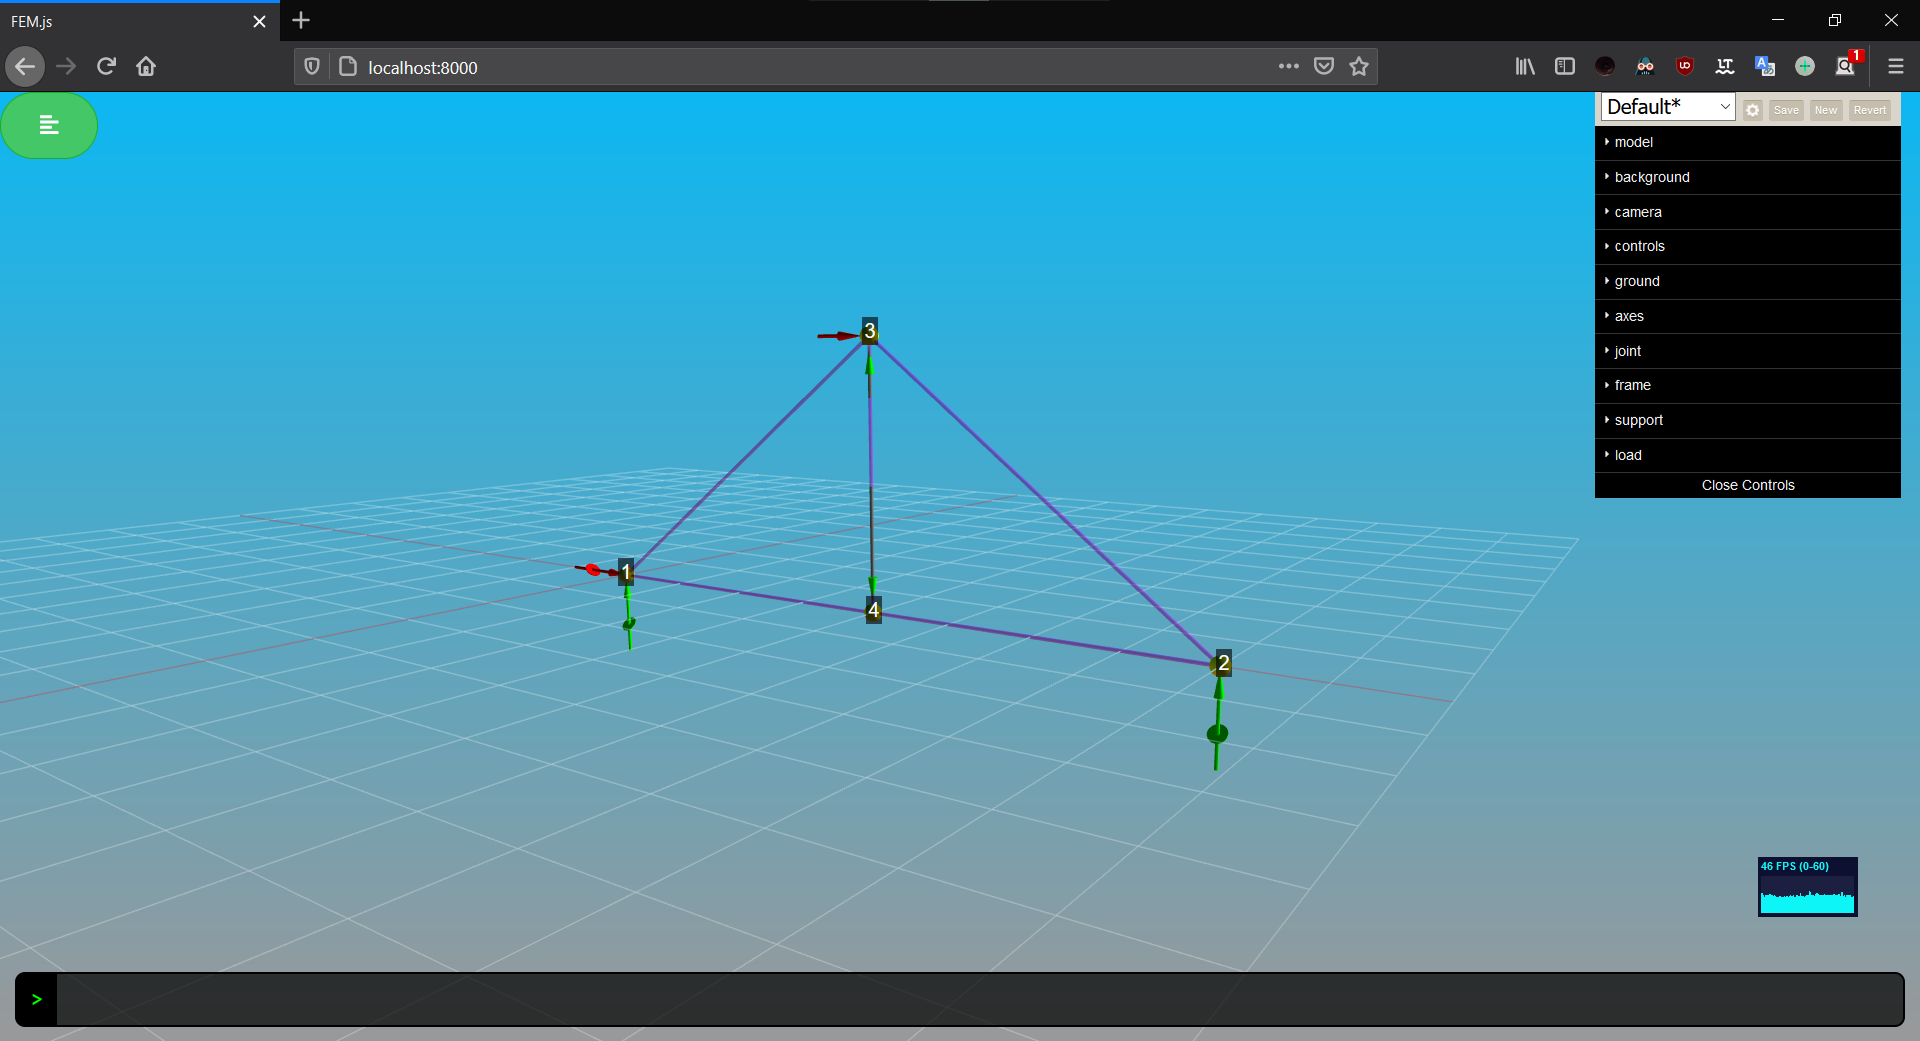
\includegraphics[width=0.8\textwidth]{introduction/FEM.js-cercha-plana.png}
  \caption{Ejemplo \ref{ej:cercha-plana} modelado en FEM.js.}
  \label{fig:FEM.js-cercha-plana}
\end{figure}

\subsubsection{dat.gui}
El panel lateral derecho de FEM.js fue desarrollado con \emph{dat.GUI} para que el usuario pueda personalizar la escena. Este panel está agrupado en las siguientes categorias:

\begin{multicols}{2}
  \begin{itemize}
  \item model,
  \item background,
  \item camera,
  \item controls,
  \item ground,
  \item axes,
  \item joint,
  \item frame,
  \item support,
  \item load.
  \end{itemize}
\end{multicols}

En la sección \verb|model| se establece la orientación del modelo al definir uno de los ejes principales del modelo que apunta hacía la parte superior de la pantalla y una subsección llamada \emph{axes}. En esta sección se define el tamaño y visibilidad de los ejes principales del modelo y dos subsecciones llamadas \emph{head} y \emph{shaft}. En estas susecciones se define la geometría de la cabeza y la cola de los vectores de los ejes principales del modelo.\\

% En la figura \ref{fig:dat.gui-model} se presenta esta sección expandida.

% \begin{figure}[ht]
%   \centering
%   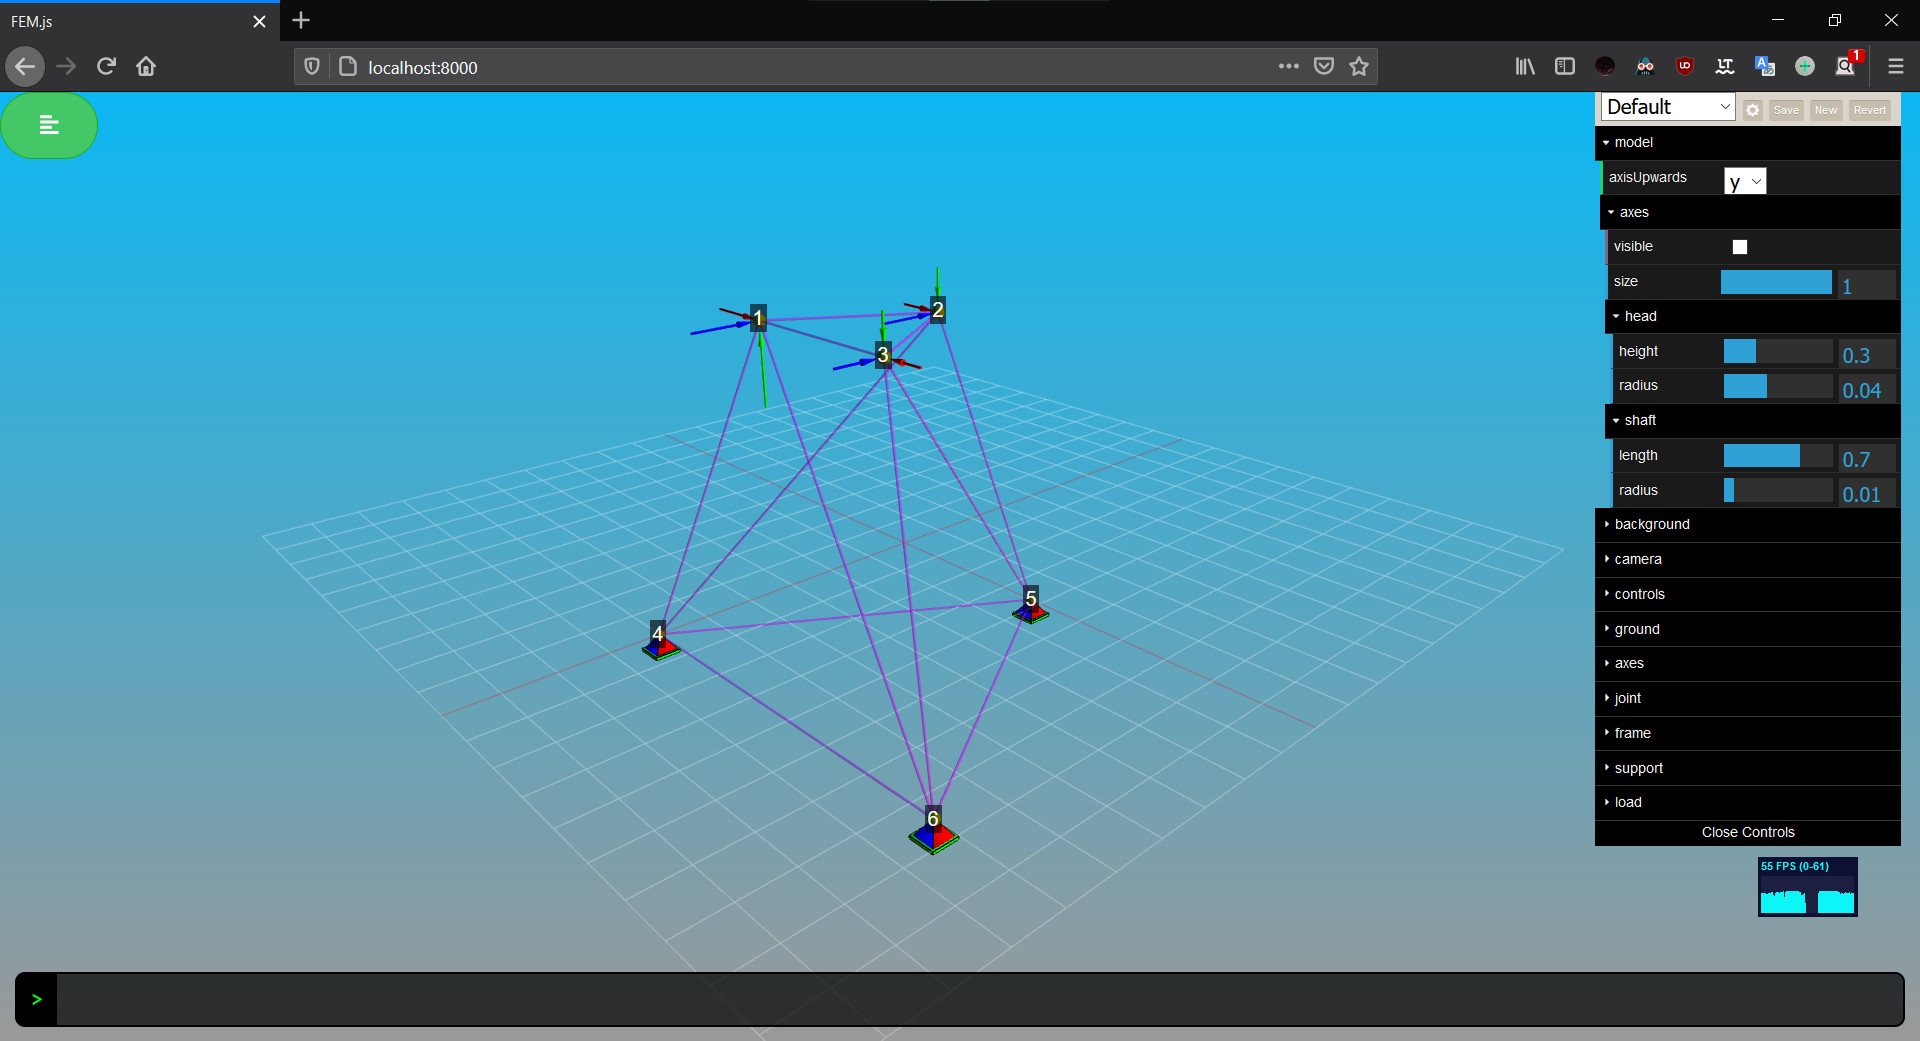
\includegraphics[width=0.8\textwidth]{introduction/dat-gui-model.png}
%   \caption{Sección \emph{model} del panel lateral de FEM.js.}
%   \label{fig:dat.gui-model}
% \end{figure}

En la sección \verb|background| se establen dos colores para generar el fondo de la escena en gradiente. El color \emph{top} define el color para la parte superior del fondo de la escena mientras que el color \emph{bottom} define el color para la parte inferior.\\

% En la figura \ref{fig:dat.gui-background} se presenta esta sección expandida.\\

% \begin{figure}[ht]
%   \centering
%   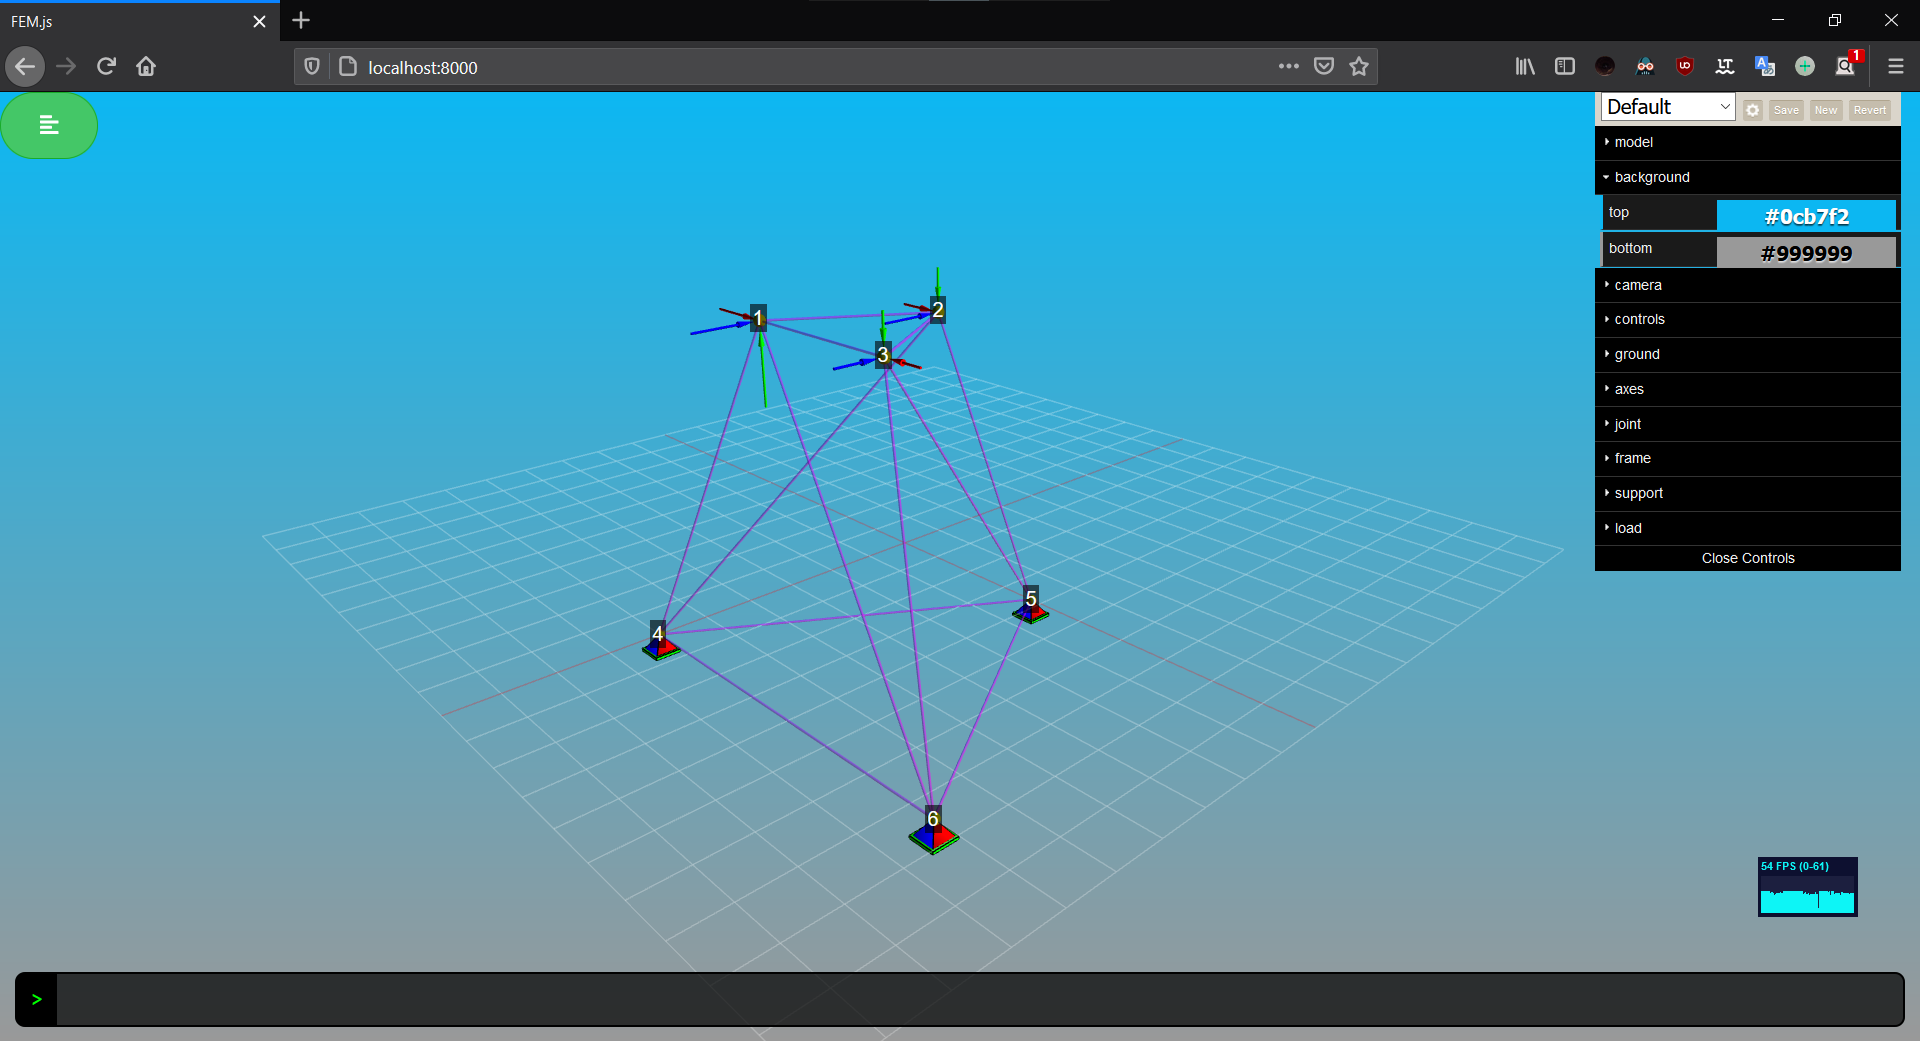
\includegraphics[width=0.8\textwidth]{introduction/dat-gui-background.png}
%   \caption{Sección \emph{background} del panel lateral de FEM.js.}
%   \label{fig:dat.gui-background}
% \end{figure}

En la sección \verb|camera| se establece el tipo de proyección de la cámara pudiéndose elegir entre perspectiva y ortogonal. En la figura \ref{fig:dat.gui-camera} se presenta el modelo del archivo \verb|example_2.json| en proyección ortogonal.\\

\begin{figure}[ht]
  \centering
  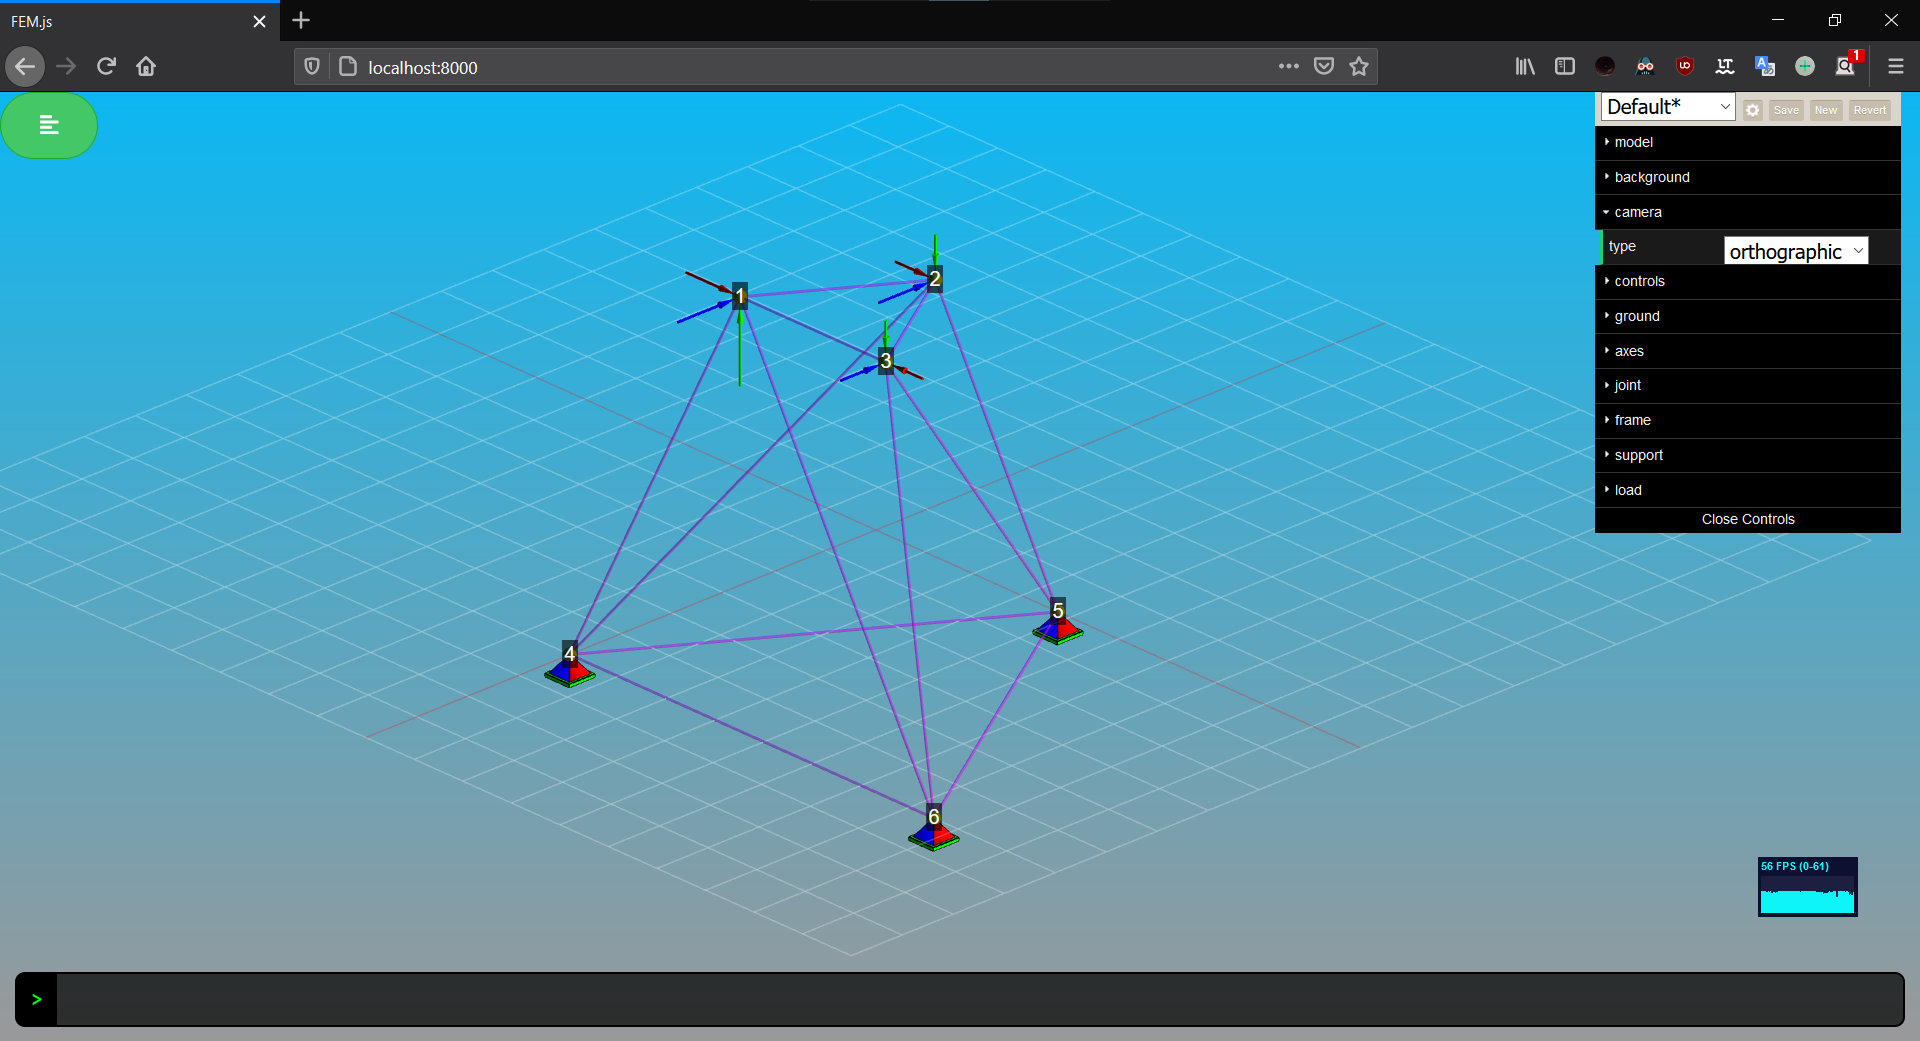
\includegraphics[width=0.8\textwidth]{introduction/dat-gui-camera.png}
  \caption{FEM.js en proyección ortogonal.}
  \label{fig:dat.gui-camera}
\end{figure}

En la sección \verb|controls| se establece el comportamiento de los controles de FEM.js. Ahí se define la velocidad con la que estos hacen rotar, hacen \emph{zoom}, desplazan la escena, si se desplaza la escena paralelo al plano del modelo o al plano de la proyección y una subsección llamada \verb|damping|. En esta subsección se define si se adiciona un \emph{amortiguamiento} a la rotación y la intensidad del mismo.\\

En la sección \verb|ground| se define la visibilidad y el tamaño del conjunto de elementos \emph{plano} y \emph{grilla} así como dos secciones llamadas \verb|plane| y \verb|grid|. En la sección \verb|plane| se define la visibilidad, el color, la transparencia y la opacidad del plano del modelo mientras que en la sección \verb|grid| se define la visibilidad, el número de divisiones y los colores de las divisiones mayores y menores de la grilla.\\

En la sección \verb|axes| se definen tres colores los cuales se asocian a los ejes $ x $, $ y $ y $ z $. Estos colores establecen los colores de los ejes globales y locales, los apoyos y las cargas. En la figura \ref{fig:dat.gui-axes} se presenta el modelo del archivo \verb|example_3.json| con una definición alternativa de dichos colores.\\

\begin{figure}[ht]
  \centering
  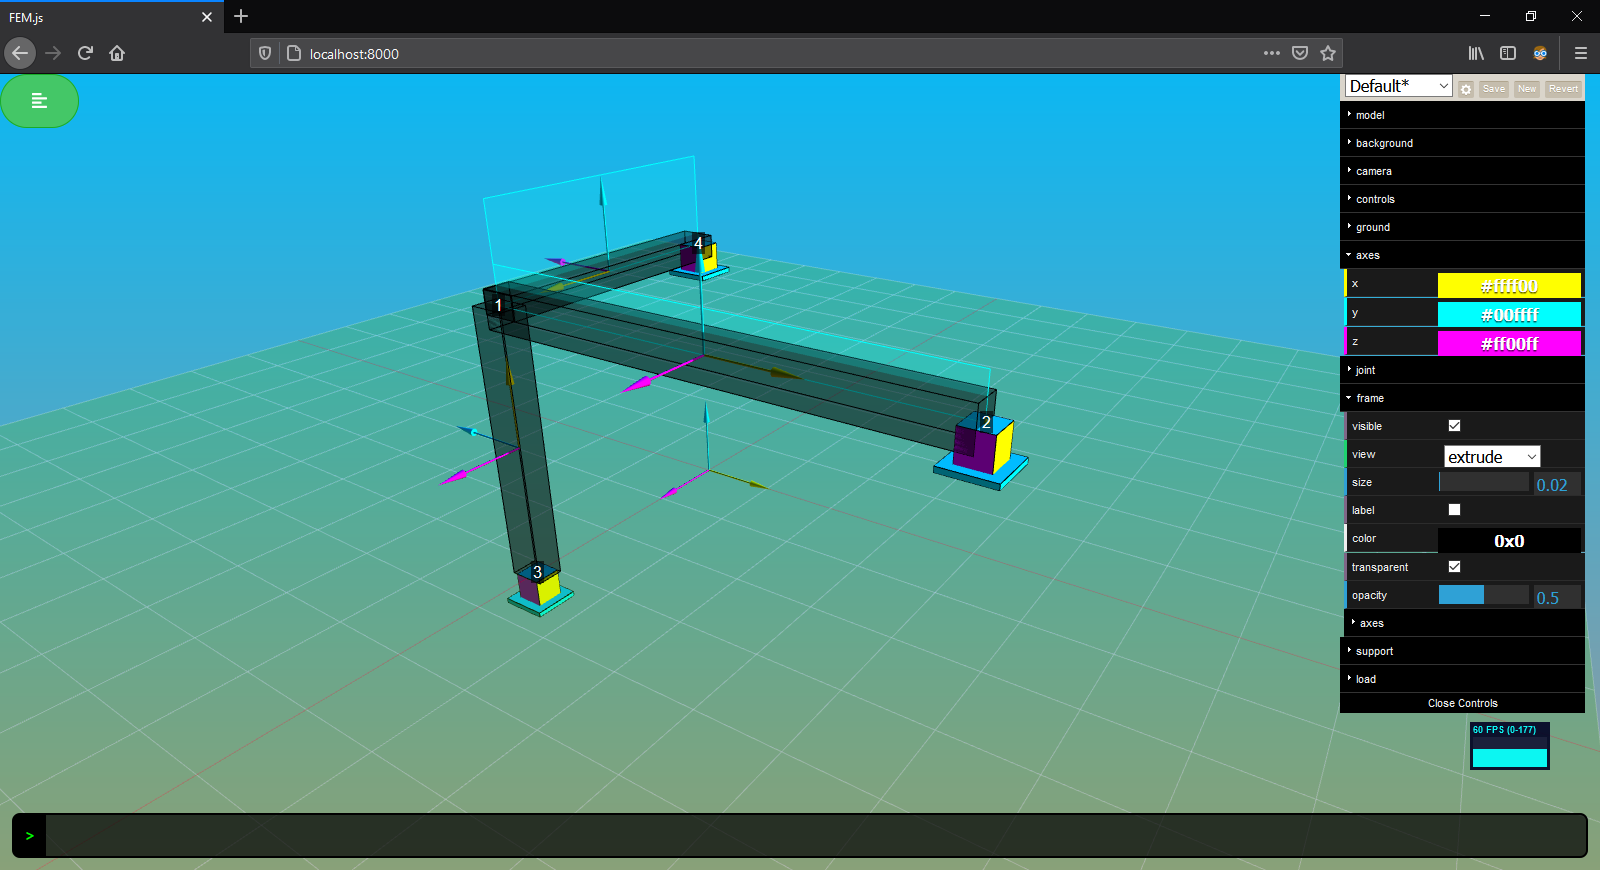
\includegraphics[width=0.8\textwidth]{introduction/dat-gui-axes.png}
  \caption{Colores alternativos para los elementos asociados a los ejes $ x $, $ y $ y $ z $.}
  \label{fig:dat.gui-axes}
\end{figure}

En la sección \verb|joint| se define la visibilidad, el tamaño, el color, la transparencia y la opacidad de los nodos del modelo. Así mismo se define la visibilidad de los \emph{labels} de los nodos.\\

En la sección \verb|frame| se define la visibilidad, la vista (\emph{extruida} o en \emph{palillo}), el tamaño, el color, la transparencia y la opacidad de los elementos tipo pórtico del modelo. Así mismo se define la visibilidad de los \emph{labels} de estos elementos y una sección llamada \verb|axes|, similar a la que se encuentra en la sección \verb|model|, con la diferencia que esta establece la visibilidad y el tamaño de los ejes locales de los elementos tipo pórtico. En la figura \ref{fig:dat.gui-frame} se presenta el modelo del archivo \verb|example_3.json| en \emph{estructura de palillo}.\\

\begin{figure}[ht]
  \centering
  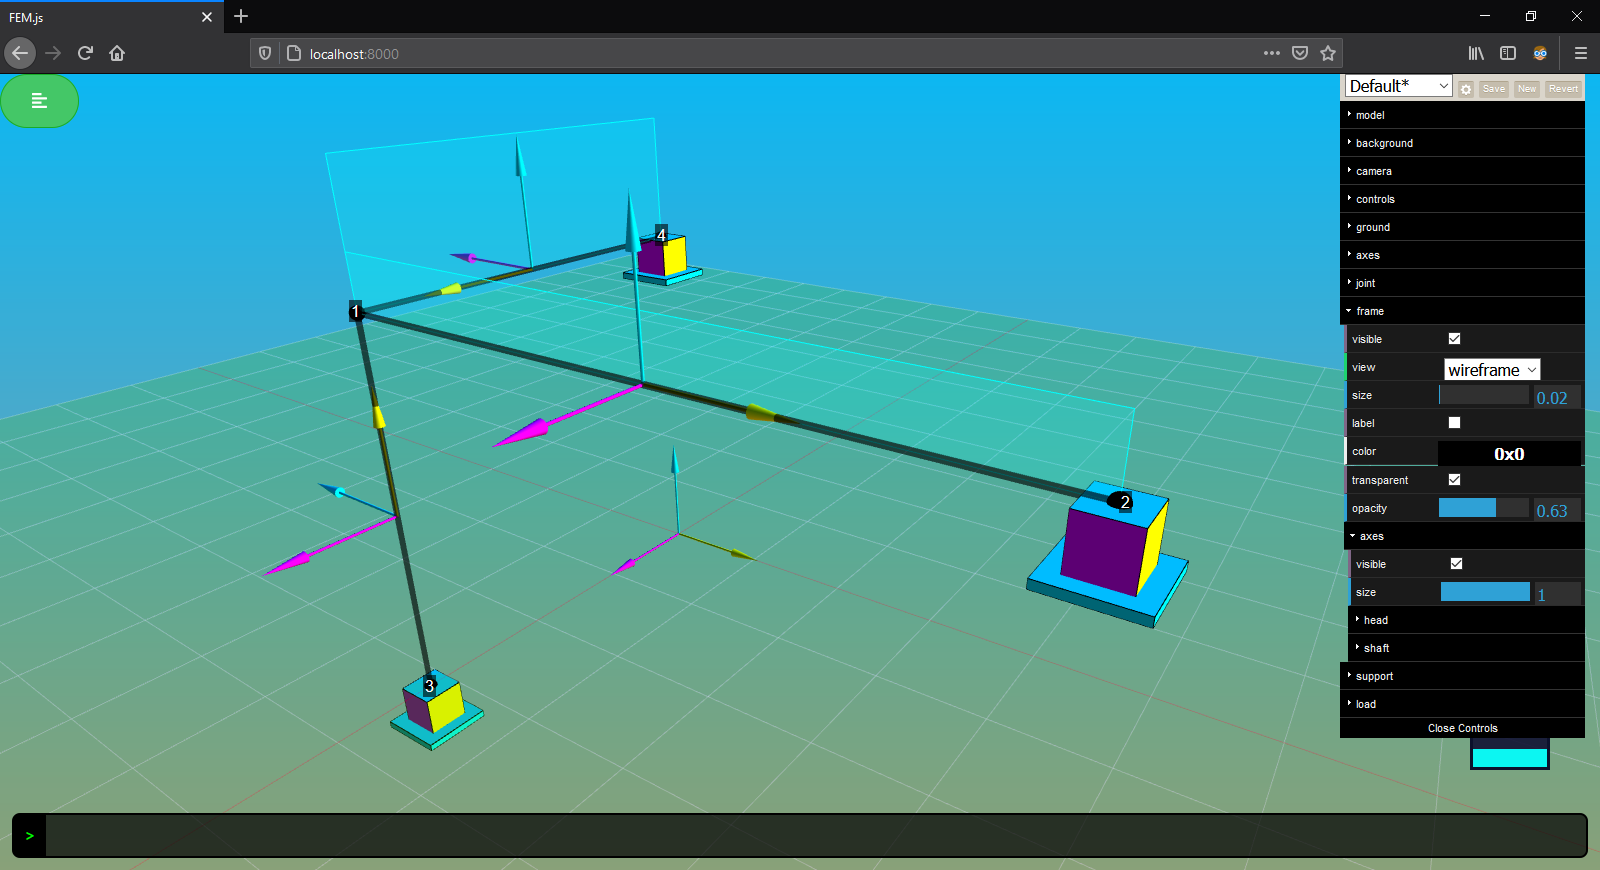
\includegraphics[width=0.8\textwidth]{introduction/dat-gui-frame.png}
  \caption{Vista del modelo como \emph{estructura de paillo}.}
  \label{fig:dat.gui-frame}
\end{figure}

En la sección \verb|support| se define la visibilidad, el \emph{modo} de los apoyos del modelo y dos secciones llamadas \verb|analytical| y \verb|space|. Los modos de los apoyos pueden ser \emph{space} o \emph{analytical}, en donde estos se representan con alguna de las analogías usadas en la literatura para representar apoyos o mediante vectores con un disco inclinado en la mitad de las colas.\\

En la sección \verb|analytical| se definen tres secciones llamadas \verb|head|, \verb|shaft| y \verb|restraint|, con las cuales se puede definir la geometría de los vectores con colas rectas o curvas (para representar restricciones a la traslación o a la rotación respectivamente) que tienen un un disco inclinado en la mitad de la cola.\\

En la sección \verb|space| se definen tres secciones llamadas \verb|foundation|, \verb|pedestal| y \verb|pin|, con las cuales se puede definir la geometría de los elementos \emph{fundación}, \emph{pedestal} o \emph{rótula}, usados para representar los apoyos como elementos espaciales. Cuando se restringen todas las traslaciones y rotaciones el apoyo se resepresenta mediante un pedestal y una fundación, mientras que si se restrigen solo las translaciones el apoyo se representa por un pedestal y una pirámide con base cuadrada. Estos apoyos toman los colores definidos en la sección \verb|axes| de manera conveniente.\\

En la figura \ref{fig:dat.gui-support} se presenta el modelo del archivo \verb|example_3.json| con los apoyos en modo \emph{analytical}.\\

\begin{figure}[ht]
  \centering
  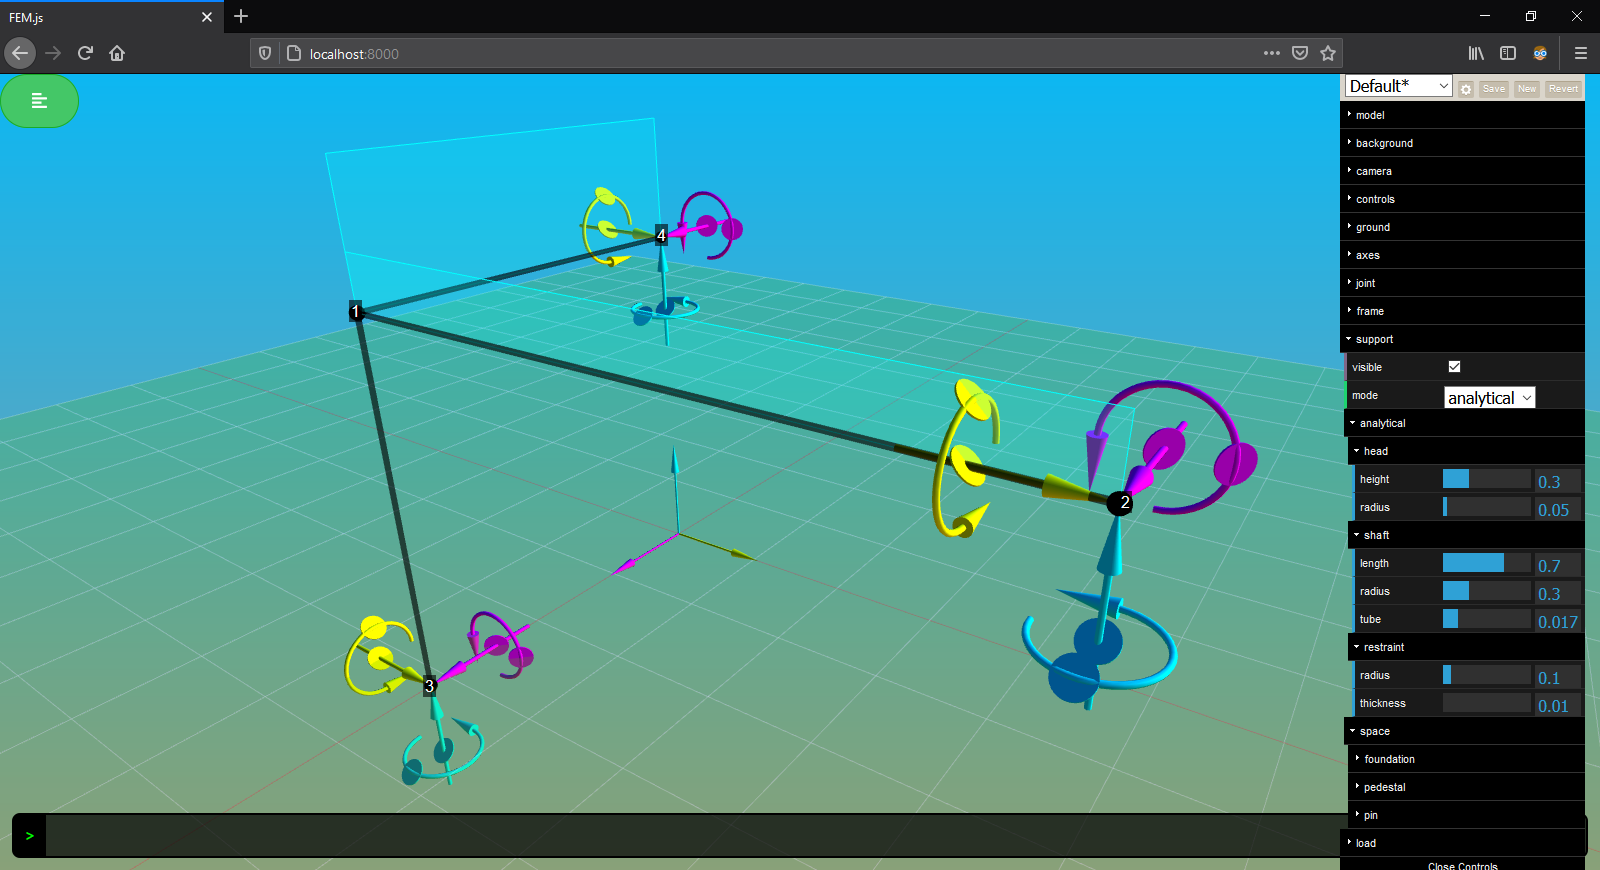
\includegraphics[width=0.8\textwidth]{introduction/dat-gui-support.png}
  \caption{Apoyos del modelo en modo \emph{analytical}.}
  \label{fig:dat.gui-support}
\end{figure}

En la sección \verb|load| se define la visibilidad, el patrón de cargas, el sistema de coordenadas de referencia y como se representan las cargas del modelo, así como cuatro secciones con los nombres \verb|force|, \verb|torque|, \verb|head| y \verb|shaft|. En el momento únicamente se cuenta con el sistemda de refencia global para representar las cargas mientras que se pueden represetar como resultantes o componentes, aunque esta última opción actualmente sólo esta disponible para las cargas puntuales.\\

En las secciones \verb|force|, \verb|torque|, \verb|head| y \verb|shaft| se definen las dimensiones y el color de los elementos que representan las cargas. El tamaño de los diferentes elementos para representar las cargas se escalan en función de valor que estas representen.\\